\chapter{Predizione semplice}
	Come già accennato nell'introduzione, per semplicità di studio, nonché per ovvi motivi, quali l'effettiva impossibilità di uno studio approfondito del fenomeno, si è ipotizzato che le chiocciole oggetto di studio siano in grado di osservare un certo numero di altezze di marea, ognuna a distanza di un numero prefissato di ore, e quindi prevedere l'altezza della marea dopo un numero arbitrario di ore.\\
	\\
	Per \textbf{predizione semplice} si intende la simulazione della predizione dell'altezza della marea futura da parte della \textit{Cerithidea decollata} in un ambiente privo di errori sensoriali, ovvero una situazione in cui la chiocciola è in grado di osservare le altezze di marea con precisione assoluta e di valutare gli intervalli temporali con altrettanta precisione.\\
	Per il codice MatLab relativo alla predizione semplice si veda il Codice \ref{lst:tideLin} a pagina \pageref{lst:tideLin}, con l'accortezza di impostare i valori di rumore sulla marea (\textit{minTN} e \textit{maxTN}) e sulle ore (\textit{minHN} e \textit{maxHN}) tutti a zero.
	\section{Predizione semplice a due ore di distanza}
		Per avvicinarsi il più possibile al comportamento della \textit{Cerithidea decollata} le prime simulazioni effettuate sono state quelle  in cui la chiocciola osserva 5 altezze di marea, ognuna a distanza di mezz'ora l'una da l'altra, per effettuare quindi la predizione di come sarà l'altezza di marea due ore dopo.\\
		\\
		Da queste simulazioni si sono ottenuti ottimi risultati: lo scarto quadratico medio raggiunto durante l'addestramento su 28 giorni è dell'ordine di \(10^{-5}\), il quale, considerando che la funzione di marea assume valori tra circa -2 e 2, e che quindi il massimo errore assoluto possibile è dell'ordine di 4, significa che in media le chiocciole sbagliano l'altezza della marea a due ore di distanza di circa lo \textbf{0,0006 \%}.\\
		\\
		Per ottenere queste simulazioni basta assegnare alle variabili \textit{int} e \textit{forecast} nel Codice \ref{lst:tideLin} i valori, rispettivamente, di \textit{0.5} e \textit{2}.\\
		Nei grafici relativi a queste simulazioni, che proponiamo di seguito la linea continua di colore blu indica la funzione di marea esatta, i punti cerchiati in blu indicano le altezze di marea osservate prima della previsione e la croce ed il cerchio rossi indicano, rispettivamente, l'altezza futura di marea prevista dalla chiocciola e quella effettiva.\\
		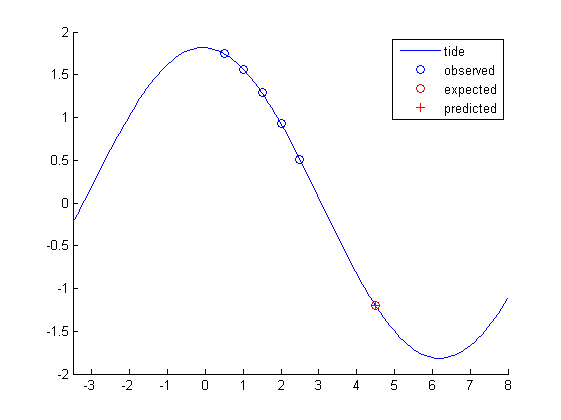
\includegraphics[width=0.6\textwidth]{simple_2h_1.png}
		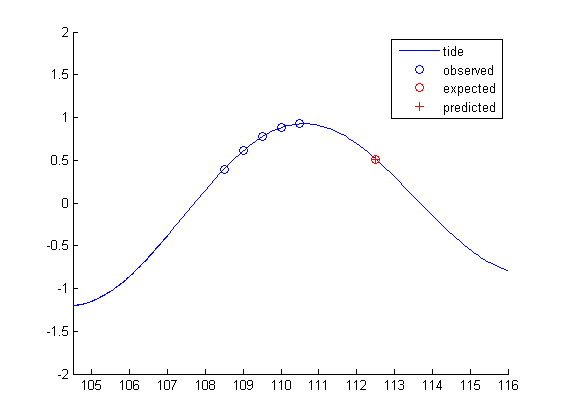
\includegraphics[width=0.6\textwidth]{simple_2h_2.png}
		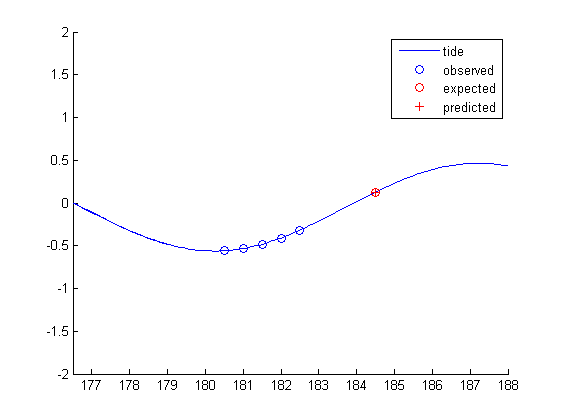
\includegraphics[width=0.6\textwidth]{simple_2h_3.png}
		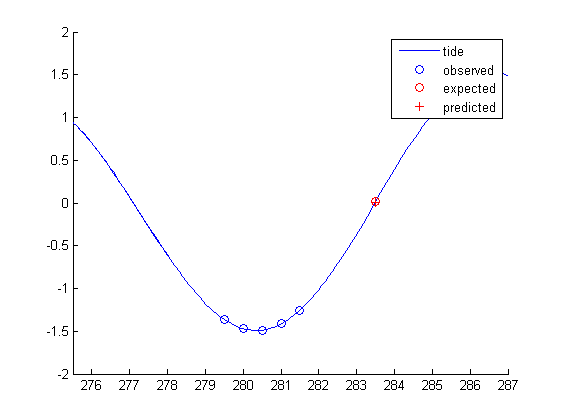
\includegraphics[width=0.6\textwidth]{simple_2h_4.png}
		\FloatBarrier
		
	\section{Predizione semplice massima}
		Per uno studio più approfondito dei limiti computazionali della rete lineare che simula il calcolo dell'altezza della marea si è provato quindi a determinare il numero massimo di ore di distanza dalla previsione, mantenendo lo scarto quadratico medio inferiore all'\textit{1\%}.\\
		\\
		Il risultato ottenuto, in via del tutto sperimentale, è di \textbf{36 ore} come intervallo massimo tra l'ultima marea osservata e la previsione che si vuole effettuare (osservando la marea ogni 2 ore) con un errore medio sull'altezza di marea inferiore all'\textbf{1\%}.
		Si noti che l'errore dell'\textit{1\%} risulta essere un valore molto basso, mentre \textit{36 ore} disponibili alla chiocciola per mettersi in salvo sul tronco di un albero sono più che sufficienti, per non dire eccessive: per errori più alti si può facilmente raggiungere un numero di ore per la previsione molto più alto, anche se inutile a fini pratici.\\
		\\
		Per riprodurre queste simulazioni basta impostare le variabili \textit{int} e \textit{forecast} a \textit{2} e \textit{36} rispettivamente (Codice \ref{lst:tideLin}).\\
		Di seguito alcuni grafici relativi a queste simulazioni:\\
		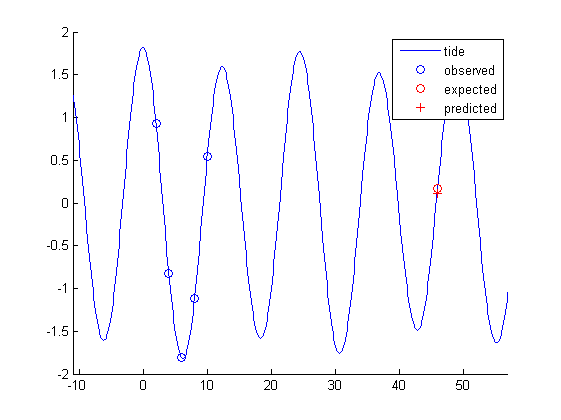
\includegraphics[width=0.6\textwidth]{simple_max_1.png}
		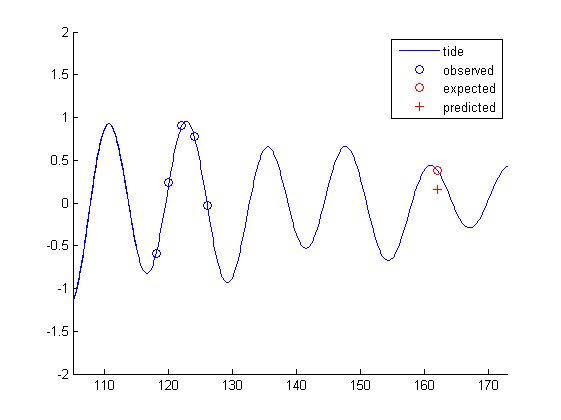
\includegraphics[width=0.6\textwidth]{simple_max_2.png}
		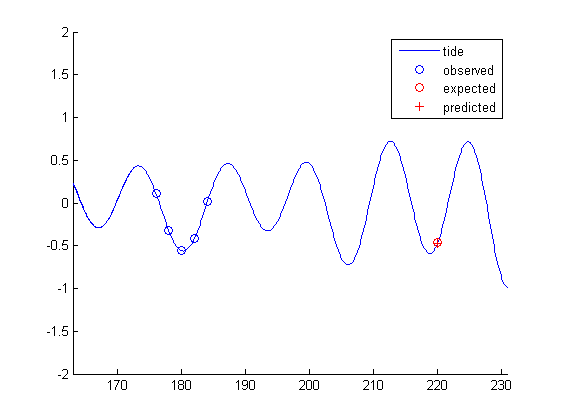
\includegraphics[width=0.6\textwidth]{simple_max_3.png}
		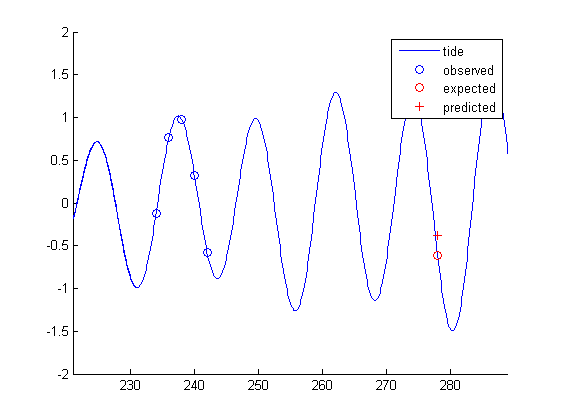
\includegraphics[width=0.6\textwidth]{simple_max_4.png}
		\FloatBarrier